% Created 2016-05-20 五 15:03
\documentclass[xcolor=svgnames,presentation]{beamer}
\usepackage[utf8]{inputenc}
\usepackage[T1]{fontenc}
\usepackage{fixltx2e}
\usepackage{graphicx}
\usepackage{longtable}
\usepackage{float}
\usepackage{wrapfig}
\usepackage{soul}
\usepackage{textcomp}
\usepackage{marvosym}
\usepackage{wasysym}
\usepackage{latexsym}
\usepackage{amssymb}
\usepackage{hyperref}
\tolerance=1000
\usepackage{minted}
\usecolortheme[named=FireBrick]{structure}\setbeamercovered{transparent}\setbeamertemplate{caption}[numbered]\setbeamertemplate{blocks}[rounded][shadow=true] \usetheme{Darmstadt}\date{\today} \usepackage{tikz}\usepackage{xeCJK}\usepackage{amsmath}\setmainfont{Times New Roman}\setCJKmainfont[BoldFont={Adobe Heiti Std},ItalicFont={Adobe Fangsong Std}]{Adobe Heiti Std}\setCJKsansfont{Adobe Heiti Std}\setCJKmonofont{Adobe Fangsong Std}\usepackage{verbatim}\graphicspath{{figures/}} \definecolor{lstbgcolor}{rgb}{0.9,0.9,0.9} \usepackage{listings}\usepackage{minted} \usepackage{fancyvrb}\usepackage{xcolor}\lstset{escapeinside=`',frameround=ftft,language=C,breaklines=true,keywordstyle=\color{blue!70},commentstyle=\color{red!50!green!50!blue!50},frame=shadowbox,backgroundcolor=\color{yellow!20},rulesepcolor=\color{red!20!green!20!blue!20}}
\usemintedstyle{default}
\providecommand{\alert}[1]{\textbf{#1}}

\title{第8讲 Linux网络与服务配置管理}
\author{王晓庆}
\date{\today}
\hypersetup{
  pdfkeywords={},
  pdfsubject={},
  pdfcreator={Emacs Org-mode version 7.9.3f}}

\institute{wangxiaoqing@outlook.com}
\begin{document}

\maketitle

\begin{frame}
\frametitle{Outline}
\setcounter{tocdepth}{1}
\tableofcontents
\end{frame}
\section{网络连接配置管理}
\label{sec-1}
\begin{frame}
\frametitle{网卡设备命名规则}
\label{sec-1-1}
\begin{itemize}

\item 网卡设备名的格式为:网卡类型+网卡序号
\label{sec-1-1-1}%

\item 以太网卡的设备名用ethN来表示,第一块以太网卡的设备名为eth0,第二块以太网卡的设备名为eth1,其余依次类推
\label{sec-1-1-2}%

\item Linux支持一块物理网卡绑定多个IP地址,此时对于每个绑定的IP地址,需要一个虚拟网卡,该网卡的设备名为ethN:M,其中N和M均为从0开始的数字
\label{sec-1-1-3}%
\end{itemize} % ends low level
\end{frame}
\begin{frame}
\frametitle{网络配置文件}
\label{sec-1-2}
\begin{itemize}

\item /etc/hosts\\
\label{sec-1-2-1}%
存储主机名和IP地址映射,用来解析无法用其他方法解析的主机名

\item /etc/resolv.conf\\
\label{sec-1-2-2}%
与域名解析有关的设置

\item /etc/sysconfig/network\\
\label{sec-1-2-3}%
定义所有网络接口的路由和主机信息

\item /etc/sysconfig/network-scripts/ifcfg-<网络接口名>\\
\label{sec-1-2-4}%
对于每个网络接口,都有一个相应的接口配置文件,提供该网络接口的特定信息
\end{itemize} % ends low level
\end{frame}
\begin{frame}[fragile]
\frametitle{网卡基本配置}
\label{sec-1-3}
\begin{itemize}

\item 编辑配置文件\\
\label{sec-1-3-1}%
\begin{minted}[]{bash}
vim /etc/sysconfig/network-scripts/ifcfg-eth0
DEVICE=eth0              #该网卡设备名称
ONBOOT=yes               #计算机启动时是否启用该网卡
BOOTPROTO=static         #启动协议(dhcp|static|none)
IPADDR=192.168.56.200    # IP地址
NETMASK=255.255.255.0    #子网掩码
HWADDR=00:0c:29:ec:a8:50 #物理地址(MAC)
GATEWAY=192.168.0.1      #默认网关地址
TYPE=Ethernet            #网卡类型
\end{minted}


\item 使用setup命令\\
\label{sec-1-3-2}%
\begin{minted}[]{bash}
setup
\end{minted}


\item 上述配置将永久生效,但需要重启网络服务才能生效\\
\label{sec-1-3-3}%
\begin{minted}[]{bash}
service network restart
\end{minted}

\end{itemize} % ends low level
\end{frame}
\begin{frame}[fragile]
\frametitle{常用网络配置命令}
\label{sec-1-4}
\begin{itemize}

\item ifconfig\\
\label{sec-1-4-1}%
\begin{minted}[]{bash}
ifconfig -a            #查看所有网络接口信息
ifconfig eth0          #查看指定网络接口信息
#配置接口地址,立即生效,但未修改配置文件
ifconfig eth0 192.168.56.201 netmask 255.255.255.0
ifconfig eth0 down|up  #激活/关闭网卡
\end{minted}


\item ifup/ifdown\\
\label{sec-1-4-2}%
\begin{minted}[]{bash}
ifup|ifdown eth0       #激活/关闭网卡
\end{minted}


\item route\\
\label{sec-1-4-3}%
\begin{minted}[]{bash}
route -n    #查看路由表(-n 不进行域名解析)
netstat -rn #查看路由表
\end{minted}

\end{itemize} % ends low level
\end{frame}
\begin{frame}[fragile]
\frametitle{配置主机名和DNS客户端}
\label{sec-1-5}
\begin{itemize}

\item 配置主机名\\
\label{sec-1-5-1}%
\begin{minted}[]{bash}
hostname           #显示主机名
hostname myserver  #设置主机名(立即生效,但非永久)
vim /etc/sysconfig/network #永久设置主机名(重启后生效)
\end{minted}


\item 配置DNS客户端\\
\label{sec-1-5-2}%
\begin{minted}[]{bash}
vim /etc/resolv.conf
nameserver 192.168.0.1 #名称服务器
nameserver 8.8.8.8
search abc.com         #DNS搜索路径
domain abc.com         #默认域名
\end{minted}

\end{itemize} % ends low level
\end{frame}
\section{网络测试与监控}
\label{sec-2}
\begin{frame}[fragile]
\frametitle{常用网络测试与监控命令}
\label{sec-2-1}
\begin{itemize}

\item ping、traceroute、netstat
\label{sec-2-1-1}%

\item sar -n DEV|EDEV|NFS|NFSD|SOCK|ALL
\label{sec-2-1-2}%

\item tcpdump\\
\label{sec-2-1-3}%
\begin{minted}[]{bash}
tcpdump [选项] [-c 数量] [-F 文件名] [-i 网络接口] 
[-r 文件名] [-s snaplen] [-T 类型] [w 文件名] [表达式]
\end{minted}

\begin{itemize}

\item tcp使用表达式过滤需要捕捉的数据包
\label{sec-2-1-3-1}%
\begin{itemize}

\item 类型:host, net, port, portrange
\label{sec-2-1-3-1-1}%

\item 方向:src, dst, dst or src, dst and src(默认)
\label{sec-2-1-3-1-2}%

\item 协议:fddi, ether, ip, arp, rarp, tcp, udp
\label{sec-2-1-3-1-3}%

\item 其他:gateway, broadcast, less, greater
\label{sec-2-1-3-1-4}%

\item 逻辑运算符:and, or, not, \&\&, ||, !
\label{sec-2-1-3-1-5}%
\end{itemize} % ends low level

\item 选项
\label{sec-2-1-3-2}%
\begin{itemize}

\item -a 将网络地址和广播地址转换为名称
\label{sec-2-1-3-2-1}%

\item -e 输出数据链路层头部信息
\label{sec-2-1-3-2-2}%

\item -n 不进行地址解析
\label{sec-2-1-3-2-3}%

\item -v 显示详细信息
\label{sec-2-1-3-2-4}%
\end{itemize} % ends low level
\end{itemize} % ends low level
\end{itemize} % ends low level
\end{frame}
\begin{frame}[fragile]
\frametitle{常用网络测试与监控命令}
\label{sec-2-2}
\begin{itemize}

\item tcpdump\\
\label{sec-2-2-1}%
\begin{minted}[]{bash}
tcpdump not (port 22 or port 23) #不捕获ssh和telnet包
tcpdump -n -i eth0 not port 22 #捕获eth0的非ssh包
tcpdump -i eth0 [src|dst] host 192.168.1.1 #过滤主机
tcpdump -i eth0 [src|dst] net 192.168 #过滤网络
tcpdump -i eth0 [src|dst] port 80 #过滤端口号
tcpdump -i eth0 -c 8 icmp #过滤协议,捕获8个包
tcpdump -i eth1 '((tcp) and (port 80) and 
((dst host 192.168.1.254) or (dst host 192.168.1.200)))'
tcpdump -i eth1 '((icmp) and ((ether dst host 
00:01:02:03:04:05)))'
tcpdump -i eth1 '((tcp) and ((dst net 192.168) and 
(not dst host 192.168.1.200)))'
man tcpdump #查看详细信息和更多例子
\end{minted}

\end{itemize} % ends low level
\end{frame}
\section{配置路由}
\label{sec-3}
\begin{frame}[fragile]
\frametitle{Linux的路由功能}
\label{sec-3-1}
\begin{itemize}

\item Linux作为网络操作系统,内核本身就提供数据包转发,支持基本的路由功能,搭配路由软件,则可以成为较为专业的路由器
\label{sec-3-1-1}%
\begin{itemize}

\item Linux主机用作软件路由器,至少需要安装两个网络接口
\label{sec-3-1-1-1}%
\end{itemize} % ends low level

\item 启用Linux内核路由转发功能
\label{sec-3-1-2}%
\begin{itemize}

\item 默认情况下内核未开启IP数据包转发功能\\
\label{sec-3-1-2-1}%
\begin{minted}[]{bash}
sysctl -w net.ipv4.ip_forward=1 #临时启用IP转发功能
vim /etc/sysctl.conf
net.ipv4.ip_forward=1           #永久开启IP转发功能
sysctl -p                       #使配置文件立即生效
\end{minted}
\end{itemize} % ends low level
\end{itemize} % ends low level
\end{frame}
\begin{frame}[fragile]
\frametitle{配置静态路由(1)}
\label{sec-3-2}
\begin{itemize}

\item 使用route命令配置静态路由\\
\label{sec-3-2-1}%
\begin{minted}[]{bash}
route add default gw 192.168.56.1 dev eth0 #添加默认路由
route del default gw 192.168.56.1 dev eth0 #删除默认路由
#添加静态路由
route add -net 192.56.76.0/24 gw 192.168.56.200
route add -net 192.56.76.0/24 dev eth0
\end{minted}

\item 使用ip route命令配置静态路由\\
\label{sec-3-2-2}%
\begin{minted}[]{bash}
ip route add 192.0.2.0/24 via 10.0.0.1 [dev eth0]
\end{minted}
\end{itemize} % ends low level
\end{frame}
\begin{frame}[fragile]
\frametitle{配置静态路由(2)}
\label{sec-3-3}
\begin{itemize}

\item 配置永久路由:/etc/sysconfig/network-scripts/route-ethn(n=0,1,2,\ldots{})
\label{sec-3-3-1}%
\begin{itemize}

\item 配置格式1\\
\label{sec-3-3-1-1}%
\begin{verbatim}
default 192.168.0.1 dev eth0
10.10.10.0/24 via 192.168.0.1 dev eth0
172.16.1.0/24 via 192.168.0.1 dev eth0
\end{verbatim}

\item 配置格式2\\
\label{sec-3-3-1-2}%
\begin{verbatim}
ADDRESS0=10.10.10.0
NETMASK0=255.255.255.0
GATEWAY0=192.168.0.1
ADDRESS1=172.16.1.0
NETMASK1=255.255.255.0
GATEWAY1=192.168.0.1
\end{verbatim}
\end{itemize} % ends low level
\end{itemize} % ends low level
\end{frame}
\begin{frame}[fragile]
\frametitle{配置静态路由(3)}
\label{sec-3-4}
\begin{itemize}

\item 配置实例\\
\label{sec-3-4-1}%
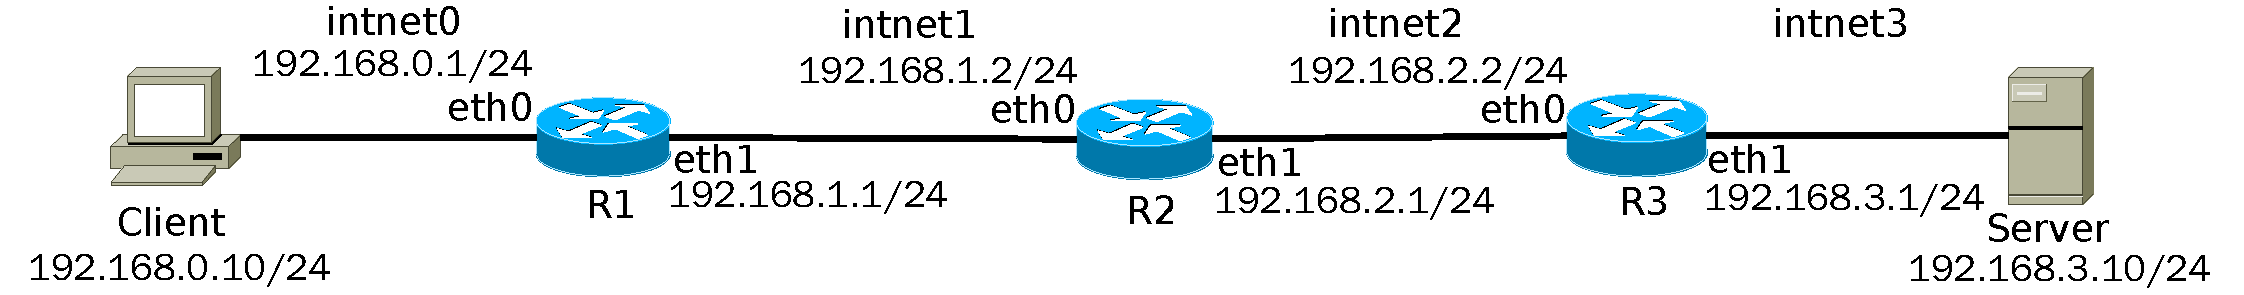
\includegraphics[width=.9\linewidth]{img/router2.pdf}

\item 配置步骤
\label{sec-3-4-2}%
\begin{itemize}
\item 配置主机和路由器的接口IP地址
\end{itemize}

\begin{minted}[]{bash}
ifconfig eth0 192.168.0.10
\end{minted}
\begin{itemize}
\item 配置主机的默认路由
\end{itemize}

\begin{minted}[]{bash}
route add default gw 192.168.0.1
\end{minted}
\begin{itemize}
\item 启用路由器的ip转发功能
\end{itemize}

\begin{minted}[]{bash}
sysctl -w net.ipv4.ip_forward=1
\end{minted}
\begin{itemize}
\item 配置路由器的静态路由
\end{itemize}

\begin{minted}[]{bash}
route add -net 192.168.3.0/24 gw 192.168.1.2
\end{minted}
\begin{itemize}
\item ping测试连通性
\end{itemize}
\end{itemize} % ends low level
\end{frame}
\begin{frame}
\frametitle{配置动态路由(1)}
\label{sec-3-5}
\begin{itemize}

\item zebra是一个开源的TCP/IP路由软件,支持主流的动态路由协议RIPvl、RIPv2、RIPng、OSPFv3、BGP-4和BGP-4+等
\label{sec-3-5-1}%

\item zebra作为软件路由器,其配置与Cisco IOS极其类似
\label{sec-3-5-2}%

\item 在实际运行中必须先启动zebra,再启动需要的动态路由协议
\label{sec-3-5-3}%

\item 在CentOS 5上安装quagga之后,/etc/init.d目录中将提供zebra相关的守护进程
\label{sec-3-5-4}%
\end{itemize} % ends low level
\end{frame}
\begin{frame}[fragile]
\frametitle{配置动态路由(2)}
\label{sec-3-6}
\begin{itemize}

\item 配置实例\\
\label{sec-3-6-1}%
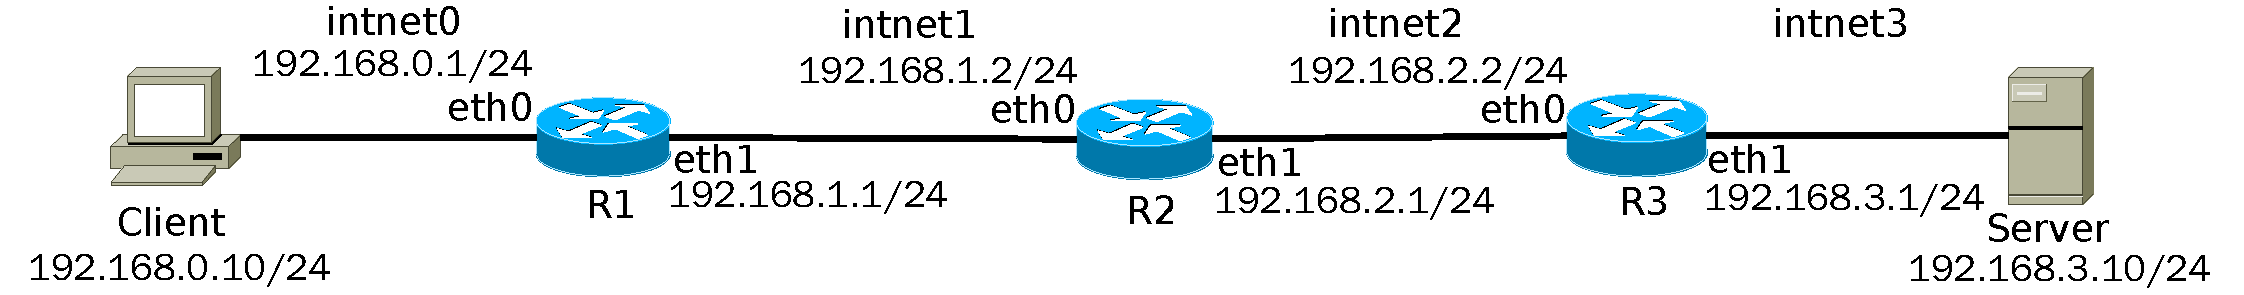
\includegraphics[width=.9\linewidth]{img/router2.pdf}

\item 配置步骤
\label{sec-3-6-2}%
\begin{itemize}

\item 安装quagga软件包
\label{sec-3-6-2-1}%

\item 安装telnet-server软件包
\label{sec-3-6-2-2}%

\item 设置zebra\\
\label{sec-3-6-2-3}%
\begin{minted}[]{bash}
vim /etc/quagga/zebra.conf #修改zebra主配置文件
hostname R1
password abc
enable password 123
!log file zebra.log
service zebra start        #启动zebra服务
telnet 127.0.0.1 2601      #本机登录zebra服务
\end{minted}
\end{itemize} % ends low level
\end{itemize} % ends low level
\end{frame}
\begin{frame}[fragile]
\frametitle{配置动态路由(3)}
\label{sec-3-7}
\begin{itemize}

\item 配置步骤(2)
\label{sec-3-7-1}%
\begin{itemize}

\item 配置RIP协议\\
\label{sec-3-7-1-1}%
\begin{minted}[]{bash}
vim /etc/quagga/ripd.conf  #配置rip服务
hostname R1
password abc
enable password 123
log stdout
router rip
  version 2
  network 192.168.0.0/24
  network 192.168.1.0/24
interface eth1 #每个rip协议接口均需配置验证
  ip rip authentication mode md5
  ip rip authentication string abc
\end{minted}
\end{itemize} % ends low level
\end{itemize} % ends low level
\end{frame}
\begin{frame}[fragile]
\frametitle{配置动态路由(4)}
\label{sec-3-8}
\begin{itemize}

\item 配置步骤(3)\\
\label{sec-3-8-1}%
\begin{minted}[]{bash}
service ripd start         #启动rip服务
telnet 127.0.0.1 2601      #登录zebra服务
show ip route
telnet 127.0.0.1 2602      #登录rip服务
enable
show ip rip
\end{minted}
\end{itemize} % ends low level
\end{frame}
\section{IPSec虚拟专用网}
\label{sec-4}
\begin{frame}
\frametitle{VPN概述(1)}
\label{sec-4-1}
\begin{itemize}

\item VPN应用模式
\label{sec-4-1-1}%
\begin{itemize}

\item 远程访问\\
\label{sec-4-1-1-1}%
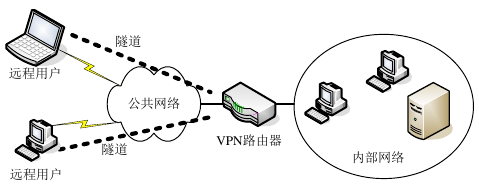
\includegraphics[width=.9\linewidth]{img/vpna.png}

\item 远程网络互联\\
\label{sec-4-1-1-2}%
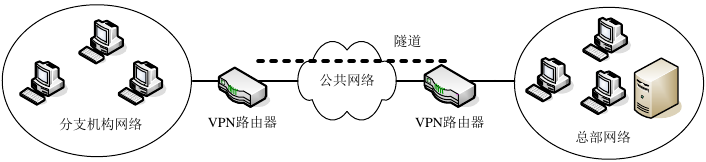
\includegraphics[width=.9\linewidth]{img/vpnb.png}
\end{itemize} % ends low level
\end{itemize} % ends low level
\end{frame}
\begin{frame}
\frametitle{VPN概述(2)}
\label{sec-4-2}
\begin{itemize}

\item 基于隧道的VPN
\label{sec-4-2-1}%
\begin{itemize}

\item 第二层隧道协议
\label{sec-4-2-1-1}%
\begin{itemize}

\item 将链路层协议封装起来进行传输,可在多种网络建立多协议的VPN,如PPTP(点对点隧道协议)和L2TP(第2层隧道协议)。
\label{sec-4-2-1-1-1}%
\end{itemize} % ends low level

\item 第三层隧道协议
\label{sec-4-2-1-2}%
\begin{itemize}

\item 用于组建IP VPN,如IPSec。IPSec工作在IP层,为IP层及其上层协议提供保护,对用户和应用程序透明,可为Internet业务提供最强的安全功能,适合于组建远程网络互联VPN。
\label{sec-4-2-1-2-1}%
\end{itemize} % ends low level

\item 第四层隧道协议
\label{sec-4-2-1-3}%
\begin{itemize}

\item 如SSL,除具备与IPSec VPN相当的安全性外,还增加访问控制机制,客户端只需要拥有支持SSL的浏览器即可,适合远程用户访问企业内部网。
\label{sec-4-2-1-3-1}%
\end{itemize} % ends low level
\end{itemize} % ends low level
\end{itemize} % ends low level
\end{frame}
\begin{frame}
\frametitle{ipsec概述}
\label{sec-4-3}
\begin{itemize}

\item IPsec基于端对端的模式来提供IP数据包的安全性,它在源IP和目的IP地址之间建立信任和安全性。
\label{sec-4-3-1}%
\begin{itemize}

\item IPsec工作在网络层(第3层),一方面可以为IP和上层协议提供保护,另一方面对于大多数应用程序、服务和高层协议是透明的。
\label{sec-4-3-1-1}%

\item IPsec使用两个安全协议AH(Authentication Header, 认证头)和ESP(Encapsulating Security Payload, 封装安全载荷),以及密钥分配的过程和相关协议来实现其目标。
\label{sec-4-3-1-2}%

\item AH可用来保证数据完整性,提供反重播保护,并且确保主机的身份验证。ESP提供和AH相似的功能,另外还提供数据机密性保护。
\label{sec-4-3-1-3}%
\end{itemize} % ends low level
\end{itemize} % ends low level
\end{frame}
\begin{frame}
\frametitle{ipsec模式}
\label{sec-4-4}
\begin{itemize}

\item ipsec有两种模式:传输模式和隧道模式,AH和ESP均可用于这两种模式。\\
\label{sec-4-4-1}%
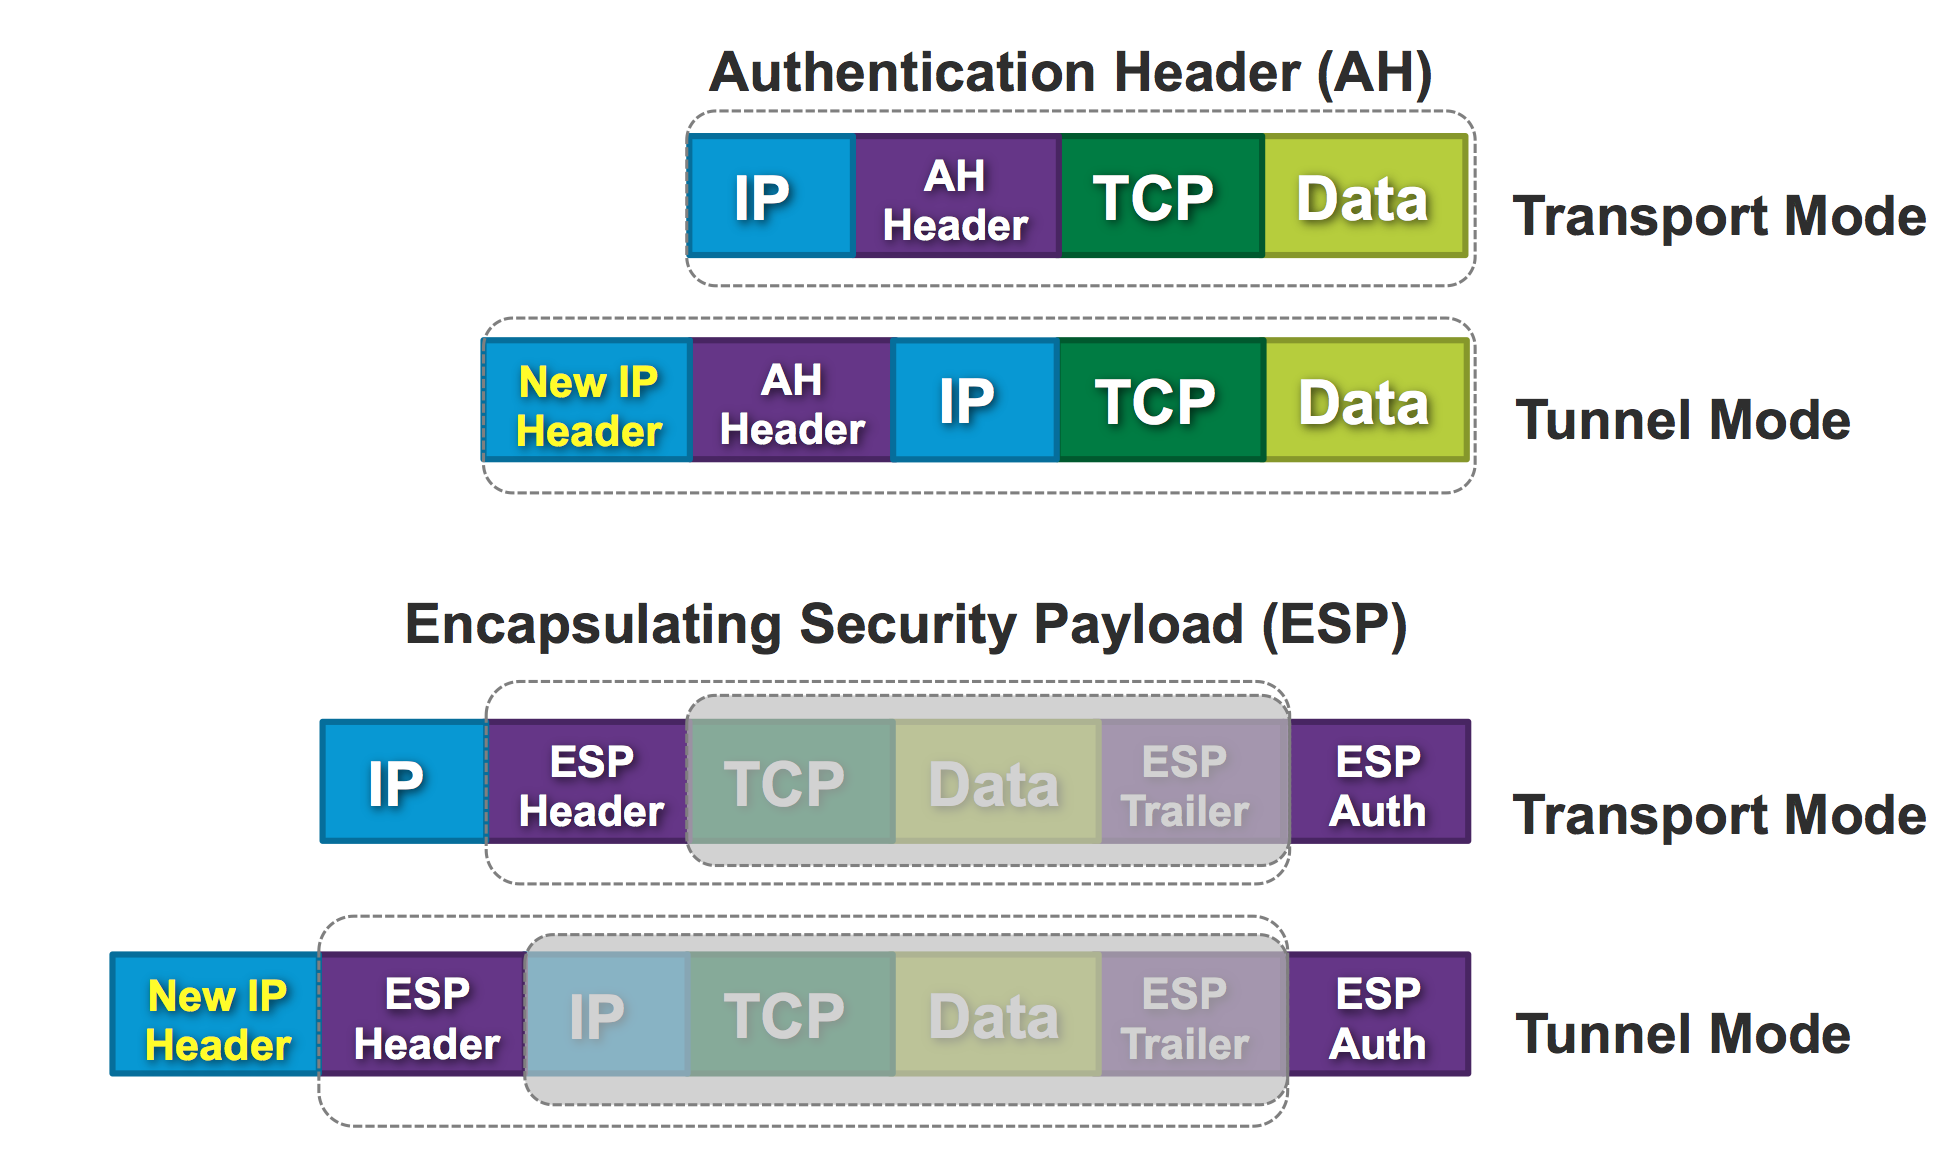
\includegraphics[width=.9\linewidth]{img/ipsec04.png}
\end{itemize} % ends low level
\end{frame}
\begin{frame}
\frametitle{ipsec安全协商}
\label{sec-4-5}
\begin{itemize}

\item 在两端实现ipsec通信之前,必须在某些安全性设置方面达成一致,主要是确定身份验证、完整性和加密算法,这个过程称为安全协商。
\label{sec-4-5-1}%

\item 安全关联(Security Association, SA)
\label{sec-4-5-2}%
\begin{itemize}

\item 安全关联存储在ipsec两端设备的数据库中,是协商密钥、安全协议与安全参数索引(spi)的组合,它们一起定义了用于保护从发送端到接收端的单向安全逻辑连接。
\label{sec-4-5-2-1}%

\item 每次ipsec通信需要建立一对SA,一个用于入站通信,一个用于出站通信。每个SA使用唯一的spi标识。如果一台设备同时与多台设备进行ipsec通信,就会存在多个SA。接收端设备使用spi来决定将使用哪个SA处理入站数据包。
\label{sec-4-5-2-2}%
\end{itemize} % ends low level

\item Internet密钥交换(Internet Key Exchange, IKE)
\label{sec-4-5-3}%
\begin{itemize}

\item IKE协议主要有两个作用:
\label{sec-4-5-3-1}%
\begin{enumerate}
\item 集中管理安全关联以减少连接时间
\item 生成和管理密钥
\end{enumerate}
\end{itemize} % ends low level
\end{itemize} % ends low level
\end{frame}
\begin{frame}
\frametitle{ipsec安全协商的两个阶段}
\label{sec-4-6}
\begin{itemize}

\item 第一阶段
\label{sec-4-6-1}%
\begin{itemize}

\item 在两端之间建立一个主模式SA(IKE SA),是为建立信道而建立的安全关联。这一阶段协商创建一个通信信道,并对该信道进行认证,为双方进一步的IKE通信提供机密性、数据完整性以及数据源认证服务。
\label{sec-4-6-1-1}%
\end{itemize} % ends low level

\item 第二阶段
\label{sec-4-6-2}%
\begin{itemize}

\item 协商一对快速模式SA(一个SA用于入站,一个SA用于出站),是为数据传输而建立的安全关联。这一阶段使用已建立的IKE SA协商建立ipsec SA,为数据交换提供ipsec服务。
\label{sec-4-6-2-1}%
\end{itemize} % ends low level
\end{itemize} % ends low level
\end{frame}
\begin{frame}
\frametitle{安全关联数据库和安全策略数据库}
\label{sec-4-7}
\begin{itemize}

\item 安全关联数据库(Security Association Database, SAD)
\label{sec-4-7-1}%
\begin{itemize}

\item 用于存放SA的有关参数:spi值、目的IP、AH/ESP、AH验证算法、AH验证密钥、ESP验证算法、ESP验证密钥、ESP加密算法、ESP加密密钥、传输/隧道模式等参数。
\label{sec-4-7-1-1}%
\end{itemize} % ends low level

\item 安全策略数据库(Security Policy Database, SPD)
\label{sec-4-7-2}%
\begin{itemize}

\item 用于存放IPSec的规则,而这些规则定义哪些流量需要使用IPSec进行保护,如:目的IP、源IP、AH/ESP协议、目的端口、源端口、传输/隧道模式等。
\label{sec-4-7-2-1}%
\end{itemize} % ends low level
\end{itemize} % ends low level
\end{frame}
\begin{frame}[fragile]
\frametitle{ipsec-tools}
\label{sec-4-8}
\begin{itemize}

\item Linux传统的ipsec解决方案是FreeS/Wan,但Linux内核从2.6版开始内置对ipsec的支持(实现了AH、ESP、SAD、SPD),并提供ipsec-tools工具来配置和管理ipsec。
\label{sec-4-8-1}%

\item ipsec-tools包括setkey和racoon两个程序
\label{sec-4-8-2}%
\begin{itemize}

\item setkey用于配置规则策略,实现SA和密钥的手动管理\\
\label{sec-4-8-2-1}%
\begin{minted}[]{bash}
setkey -f FILE #根据FILE设置SAD和SPD
setkey -D      #查看SAD
setkey -P -D   #查看SPD
setkey -F      #清空SAD
setkey -P -F   #情况SPD
man setkey     #了解详细信息
\end{minted}

\item racoon用于密钥协商,是一种IKE实现,实现SA和密钥的自动管理
\label{sec-4-8-2-2}%
\end{itemize} % ends low level
\end{itemize} % ends low level
\end{frame}
\begin{frame}
\frametitle{ipsec-tools数据处理模型}
\label{sec-4-9}
\begin{columns}
\begin{column}{0.4\textwidth}
\begin{itemize}

\item 数据处理过程\\
\label{sec-4-9-1}%
对进出数据首先确定其安全策略,如果需要安全服务,则找到对应的SA,根据SA相关参数进行AH/ESP封装后再完成数据的输入/输出。
\end{itemize} % ends low level
\end{column}
\begin{column}{0.6\textwidth}
%% ipsec-tools的处理模型
\label{sec-4-9-2}

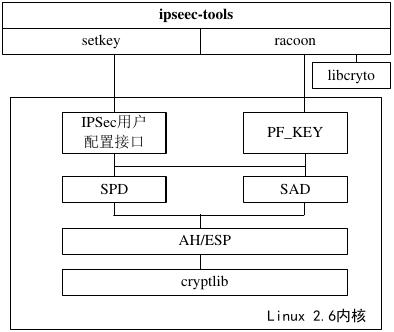
\includegraphics[width=.9\linewidth]{img/ipsec-tools.png}
\end{column}
\end{columns}
\end{frame}
\begin{frame}[fragile]
\frametitle{配置主机到主机的ipsec连接(1)}
\label{sec-4-10}

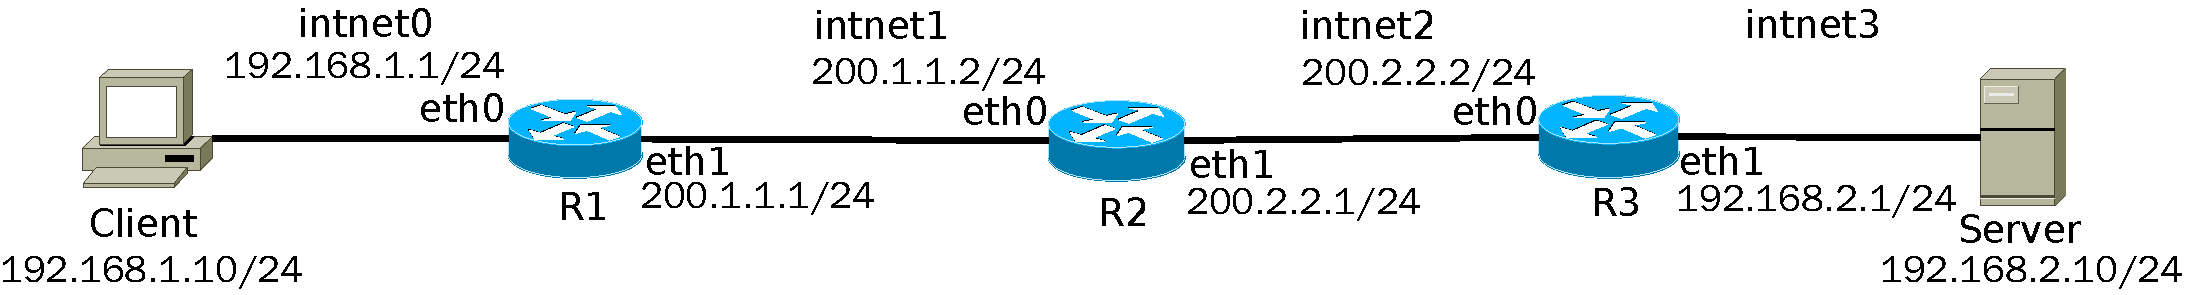
\includegraphics[width=.9\linewidth]{img/vpnlab.pdf}
\begin{itemize}

\item 配置步骤(以Client端为例,Server端类似)
\label{sec-4-10-1}%
\begin{itemize}

\item 1. 编辑ipsec接口配置文件\\
\label{sec-4-10-1-1}%
\begin{minted}[]{bash}
vim /etc/sysconfig/network-scripts/ifcfg-ipsec0
DST=192.168.2.10 #对端主机IP地址
TYPE=IPSEC       #接口类型
ONBOOT=no        #系统启动时是否激活
IKE_METHOD=PSK   #IKE验证方式(此处采用预共享密钥)
\end{minted}

\item 2. 编辑预共享密钥文件\\
\label{sec-4-10-1-2}%
\begin{minted}[]{bash}
vim /etc/sysconfig/network-scripts/keys-ipsec0
IKE_PSK=Abc_123
#为保障密码安全,最好修改keys-ipsec0的权限
chmod 600 /etc/sysconfig/network-scripts/keys-ipsec0
\end{minted}
\end{itemize} % ends low level
\end{itemize} % ends low level
\end{frame}
\begin{frame}[fragile]
\frametitle{配置主机到主机的ipsec连接(2)}
\label{sec-4-11}
\begin{itemize}

\item 配置步骤(以Client端为例,Server端类似)(续)
\label{sec-4-11-1}%
\begin{itemize}

\item 3. 重启网络服务\\
\label{sec-4-11-1-1}%
\begin{minted}[]{bash}
service network restart
\end{minted}

\item 4. Server端类似执行1~3步
\label{sec-4-11-1-2}%

\item 5. 在Client和Server上激活ipsec0接口\\
\label{sec-4-11-1-3}%
\begin{minted}[]{bash}
ifup ipsec0 #将自动生成/etc/raccoon/192.168.2.10.conf
\end{minted}

\item 6. 测试并用tcpdump抓包验证\\
\label{sec-4-11-1-4}%
\begin{minted}[]{bash}
client: ping -c 4 192.168.2.10
server: tcpdump -i eth0
\end{minted}
\end{itemize} % ends low level
\end{itemize} % ends low level
\end{frame}
\begin{frame}[fragile]
\frametitle{配置网络到网络的ipsec连接(1)}
\label{sec-4-12}

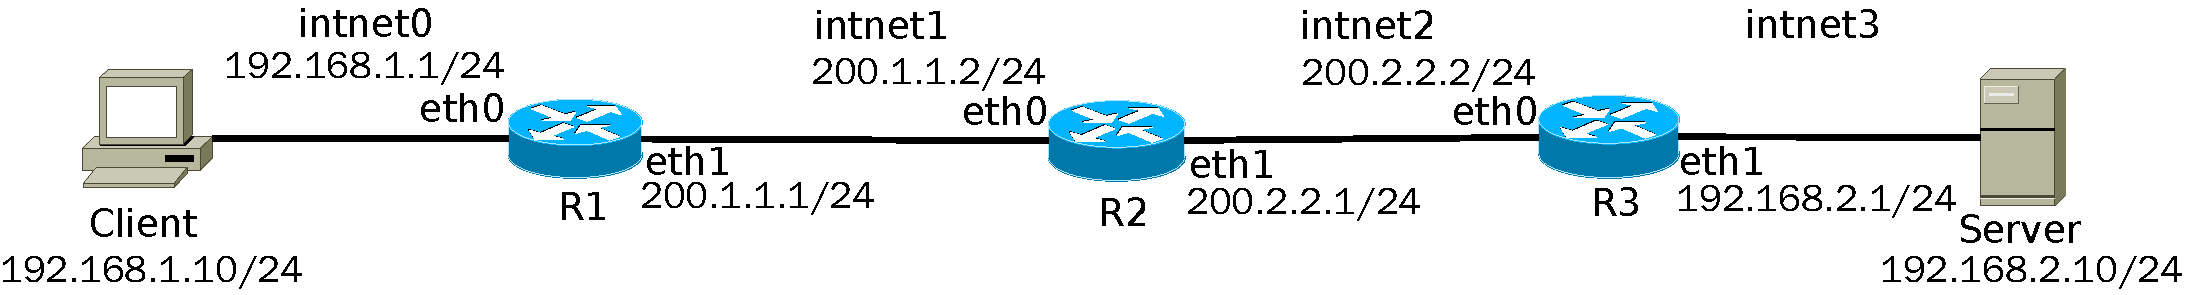
\includegraphics[width=.9\linewidth]{img/vpnlab.pdf}
\begin{itemize}

\item 配置步骤(以R1为例,R3类似)
\label{sec-4-12-1}%
\begin{itemize}

\item 1. 编辑ipsec接口配置文件\\
\label{sec-4-12-1-1}%
\begin{minted}[]{bash}
vim /etc/sysconfig/network-scripts/ifcfg-ipsec1
TYPE=IPSEC
ONBOOT=yes
IKE_METHOD=PSK
SRCGW=192.168.1.1      #源网关地址
DSTGW=192.168.2.1      #目的网关地址
SRCNET=192.168.1.0/24  #源网络
DSTNET=192.168.2.0/24  #目的网络
DST=200.2.2.2          #隧道对端公网地址
\end{minted}
\end{itemize} % ends low level
\end{itemize} % ends low level
\end{frame}
\begin{frame}[fragile]
\frametitle{配置网络到网络的ipsec连接(2)}
\label{sec-4-13}
\begin{itemize}

\item 配置步骤(以R1为例,R3类似)(续)
\label{sec-4-13-1}%
\begin{itemize}

\item 2. 编辑预共享密钥文件\\
\label{sec-4-13-1-1}%
\begin{minted}[]{bash}
vim /etc/sysconfig/network-scripts/keys-ipsec0
IKE_PSK=Abc_123
chmod 600 /etc/sysconfig/network-scripts/keys-ipsec0
\end{minted}

\item 3. 确保R1启用了ip转发功能\\
\label{sec-4-13-1-2}%
\begin{minted}[]{bash}
sysctl -a | grep ip_forward
\end{minted}

\item 4. 在R3上类似执行1~3步
\label{sec-4-13-1-3}%

\item 5. 在R1和R3上激活ipsec1接口\\
\label{sec-4-13-1-4}%
\begin{minted}[]{bash}
ifup ipsec1 #将自动生成/etc/raccoon/200.2.2.2.conf
\end{minted}

\item 6. 测试并用tcpdump抓包验证\\
\label{sec-4-13-1-5}%
\begin{minted}[]{bash}
client: ping -c 4 192.168.2.10
    R3: tcpdump -i eth0
server: tcpdump -i eth0
\end{minted}
\end{itemize} % ends low level
\end{itemize} % ends low level
\end{frame}
\section{Linux服务管理}
\label{sec-5}
\begin{frame}
\frametitle{服务的类型}
\label{sec-5-1}
\begin{itemize}

\item 按功能分
\label{sec-5-1-1}%
\begin{itemize}

\item 系统服务:指那些为系统本身或者系统用户提供的一类服务,如提供作业调度服务的cron服务。
\label{sec-5-1-1-1}%

\item 网络服务:网络服务是指供客户端调用的一类服务,如Web服务、文件服务等。
\label{sec-5-1-1-2}%
\begin{itemize}

\item 网络服务定义文件:/etc/services
\label{sec-5-1-1-2-1}%
\end{itemize} % ends low level
\end{itemize} % ends low level

\item 按启动方式分
\label{sec-5-1-2}%
\begin{itemize}

\item 独立服务(Standalone Service):启动后始终在后台执行,除非关闭系统或强制中止。多数服务属于此种类型。
\label{sec-5-1-2-1}%

\item 临时服务(Transient Service):只有当客户端需要时才会被启动,使用完毕就会结束。
\label{sec-5-1-2-2}%
\begin{itemize}

\item 超级服务xinetd用于管理其他临时服务
\label{sec-5-1-2-2-1}%
\end{itemize} % ends low level
\end{itemize} % ends low level
\end{itemize} % ends low level
\end{frame}
\begin{frame}[fragile]
\frametitle{服务控制脚本}
\label{sec-5-2}
\begin{itemize}

\item 以rpm包方式安装的服务的控制脚本统一放置在目录/etc/rc.d/init.d目录
\label{sec-5-2-1}%

\item 利用服务控制脚本控制服务\\
\label{sec-5-2-2}%
\begin{minted}[]{bash}
/etc/rc.d/init.d/sshd \
start|stop|restart|reload|condrestart|status
reload      #在不重新启动服务的前提下重新加载其配置文件
condrestart #只有服务正在运行时才重新启动该服务
service sshd start|stop|...
\end{minted}
\end{itemize} % ends low level
\end{frame}
\begin{frame}[fragile]
\frametitle{配置服务器是否自动启动}
\label{sec-5-3}
\begin{itemize}

\item 以rpm包方式安装的服务可用chkconfig或ntsysv命令配置其是否启动
\label{sec-5-3-1}%
\begin{itemize}

\item chkconfig命令\\
\label{sec-5-3-1-1}%
\begin{minted}[]{bash}
chkconfig --list      #查看所有服务的启动配置
chkconfig --list sshd #查看sshd服务的启动配置
chkconfig --level 234 sshd on #运行级别234启动sshd
chkconfig --level 24 sshd off #运行级别24关闭sshd
\end{minted}

\item ntsysv命令\\
\label{sec-5-3-1-2}%
\begin{minted}[]{bash}
ntsysv             #对当前运行级别下的服务进行启动配置
ntsysv --level 235 #对运行级别235下的服务进行启动配置
setup          #可以通过setup命令对服务进行启动配置
\end{minted}
\end{itemize} % ends low level
\end{itemize} % ends low level
\end{frame}
\section{PAM认证}
\label{sec-6}
\begin{frame}
\frametitle{PAM}
\label{sec-6-1}
\begin{itemize}

\item 为了解决多个应用的用户认证问题,Linux引入了一套名为可插拔认证模块(Pluggable Authentication Modules, PAM)的用户认证机制,将用户认证功能从应用中独立出来,单独进行模块化设计,统一实现和维护,并提供了一套标准API,以便各应用程序能够方便地使用它们所提供的各种功能。
\label{sec-6-1-1}%

\item PAM为了提供足够高的通用性、灵活性和可配置性,采用了插件机制,并采用了分层的体系结构。
\label{sec-6-1-2}%
\end{itemize} % ends low level
\end{frame}
\begin{frame}[fragile]
\frametitle{PAM认证机制(1)}
\label{sec-6-2}
\begin{itemize}

\item PAM认证过程
\label{sec-6-2-1}%
\begin{enumerate}
\item 采用PAM认证的服务或应用程序向PAM库提出验证请求,PAM实际上是一个名为libpam.so的共享链接库。
\end{enumerate}

\begin{minted}[]{bash}
ldd /bin/login | grep libpam.so #查看应用是否包含PAM库
\end{minted}
\begin{enumerate}
\item PAM库确定提出请求的是哪一项服务或应用程序,然后到/etc/pam.d目录下加载相应服务或应用程序的PAM的配置文件(与服务或应用程序同名,如vsftpd服务的配置文件为/etc/pam.d/vsftpd)。
\item PAM库根据PAM配置文件的设置调用指定的认证模块(位于/lib/security目录下)进行安全认证。
\item PAM库将认证结果返回给服务或应用程序。
\end{enumerate}
\end{itemize} % ends low level
\end{frame}
\begin{frame}
\frametitle{PAM认证机制(2)}
\label{sec-6-3}
\begin{itemize}

\item PAM体系架构\\
\label{sec-6-3-1}%
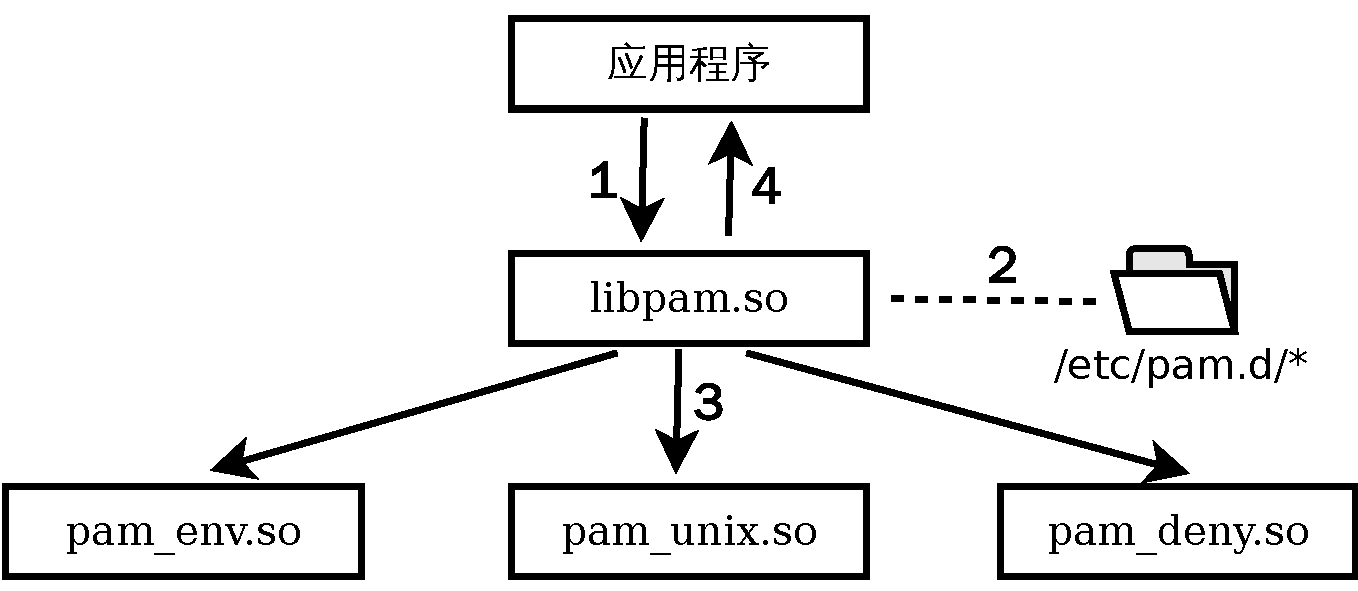
\includegraphics[width=.9\linewidth]{img/pam4.pdf}
\end{itemize} % ends low level
\end{frame}
\begin{frame}
\frametitle{PAM认证机制(3)}
\label{sec-6-4}
\begin{itemize}

\item PAM客户端可以请求PAM内核执行下列动作:
\label{sec-6-4-1}%
\begin{itemize}

\item 确认用户身份
\label{sec-6-4-1-1}%

\item 取得账户信息
\label{sec-6-4-1-2}%

\item 修改验证的凭证或帐号数据
\label{sec-6-4-1-3}%
\end{itemize} % ends low level

\item 每个PAM模块执行后都会返回success或fail,PAM内核(libpam.so)再根据该结果及PAM客户端配置文件的配置决定下一步动作。当PAM内核执行完所需执行的模块后,把最终结果返回给PAM客户端,PAM客户端则由该结果判断验证过程是否成功。
\label{sec-6-4-2}%

\item 注意:如果PAM找不到指定模块,或者PAM模块无法顺利执行,则PAM内核和PAM模块的默认返回结果都是fail。
\label{sec-6-4-3}%
\end{itemize} % ends low level
\end{frame}
\begin{frame}[fragile]
\frametitle{PAM客户端配置文件(1)}
\label{sec-6-5}
\begin{itemize}

\item 每个支持PAM的应用程序或服务都在/etc/pam.d目录中有一个相应的配置文件,其文件名与相应的应用程序或服务同名。
\label{sec-6-5-1}%

\item PAM客户端配置文件格式\\
\label{sec-6-5-2}%
\begin{verbatim}
类型 控制标记 模块路径 [模块参数]
\end{verbatim}

\item PAM认证过程根据客户端配置文件内容顺序执行。
\label{sec-6-5-3}%
\end{itemize} % ends low level
\end{frame}
\begin{frame}
\frametitle{PAM客户端配置文件(2)}
\label{sec-6-6}
\begin{itemize}

\item 类型
\label{sec-6-6-1}%
\begin{itemize}

\item auth\\
\label{sec-6-6-1-1}%
认证管理,对用户的身份进行识别,如提示用户输入密码。

\item account\\
\label{sec-6-6-1-2}%
账户管理,对账户各项属性进行检查,如是否允许登录,限制最大用户数。

\item password\\
\label{sec-6-6-1-3}%
密码管理,更新密码和凭证等,如修改用户密码。

\item session\\
\label{sec-6-6-1-4}%
会话管理,定义用户登录前和退出后要进行的操作,如显示登录连接信息。
\end{itemize} % ends low level
\end{itemize} % ends low level
\end{frame}
\begin{frame}
\frametitle{PAM客户端配置文件(3)}
\label{sec-6-7}
\begin{itemize}

\item 控制标记(1)
\label{sec-6-7-1}%
\begin{itemize}

\item required\\
\label{sec-6-7-1-1}%
表示该模块认证成功是用户通过认证的必要条件。只要模块认证失败,用户就一定不会通过认证。但即便失败,PAM也不会立即将结果返回给应用,而是继续调用其他模块。这样做的目的就是为了麻痹“敌人”,让他们搞不清楚到底是哪个环节认证失败的。

\item requisite\\
\label{sec-6-7-1-2}%
与required类似,但是只要requisite模块认证失败,就会立即返回给应用。一般用于判定当前用户所处的环境,如果环境不够安全,即便是合法的用户也不会通过验证。这是最严苛的要求,一般很少使用。但是requisite能够将低黑客利用不安全媒介获得输入密码的机会。
\end{itemize} % ends low level
\end{itemize} % ends low level
\end{frame}
\begin{frame}
\frametitle{PAM客户端配置文件(4)}
\label{sec-6-8}
\begin{itemize}

\item 控制标记(2)
\label{sec-6-8-1}%
\begin{itemize}

\item sufficient\\
\label{sec-6-8-1-1}%
表示该模块验证成功是用户通过认证的充分条件。只要这个模块验证成功了,就代表没有必要继续去认证其他模块了,将立即返回给应用。但是其优先级低于required,如果其前面有required模块失败,则最终结果也是失败,当sufficient认证失败时,相当于optional。

\item optional\\
\label{sec-6-8-1-2}%
表示即便该模块认证失败,用户也可能通过认证,除非别无它选。实际应用中,optional模块只是显示相关信息,根本不做认证工作。

\item include\\
\label{sec-6-8-1-3}%
执行指定PAM客户端配置文件中与类型字段匹配的那些模块
\end{itemize} % ends low level
\end{itemize} % ends low level
\end{frame}
\begin{frame}[fragile]
\frametitle{PAM客户端配置文件(5)}
\label{sec-6-9}
\begin{itemize}

\item system-auth配置文件
\label{sec-6-9-1}%
\begin{itemize}

\item 几乎每一个PAM客户端都会包含以下设置\\
\label{sec-6-9-1-1}%
\begin{verbatim}
auth     include system-auth
account  include system-auth
password include system-auth
session  include system-auth
\end{verbatim}

\item 因为许多应用程序会利用PAM进行验证授权,且要执行的动作几乎一样,system-auth为此提供了一个全局默认配置,如果需要修改所有PAM客户端默认的验证授权配置,只需修改system-auth文件,无需逐个修改每一个PAM配置文件。\\
\label{sec-6-9-1-2}%
\begin{minted}[]{bash}
cat /etc/pam.d/system-auth
\end{minted}
\end{itemize} % ends low level
\end{itemize} % ends low level
\end{frame}
\begin{frame}
\frametitle{常用PAM模块(1)}
\label{sec-6-10}
\begin{itemize}

\item pam\_unix.so模块(1)\\
\label{sec-6-10-1}%
该模块利用名称服务切换器取得帐号数据,然后用帐号数据进行验证授权动作。
\begin{itemize}

\item pam\_unix.so模块用于不同类型时执行不同的动作
\label{sec-6-10-1-1}%
\begin{itemize}

\item auth     以NSS解析所得的密码进行身分验证
\label{sec-6-10-1-1-1}%

\item account  以NSS解析所得的密码数据判断密码与帐号是否过期
\label{sec-6-10-1-1-2}%

\item password 将修改后的密码存储至本机或NIS服务器
\label{sec-6-10-1-1-3}%

\item session  记录登录、注销信息
\label{sec-6-10-1-1-4}%
\end{itemize} % ends low level
\end{itemize} % ends low level
\end{itemize} % ends low level
\end{frame}
\begin{frame}
\frametitle{常用PAM模块(2)}
\label{sec-6-11}
\begin{itemize}

\item pam\_unix.so模块(2)
\label{sec-6-11-1}%
\begin{itemize}

\item 常用参数
\label{sec-6-11-1-1}%
\begin{itemize}

\item debug 产生除错信息
\label{sec-6-11-1-1-1}%

\item use$_{\mathrm{first}}$$_{\mathrm{pass}}$ 如果同时使用多种验证方法,则以第一顺位的为准
\label{sec-6-11-1-1-2}%

\item try$_{\mathrm{first}}$$_{\mathrm{pass}}$ 除非没有设置PAM$_{\mathrm{AUTHTOK}}$,否则不提示用户输入密码
\label{sec-6-11-1-1-3}%

\item use$_{\mathrm{authok}}$ 与try$_{\mathrm{first}}$$_{\mathrm{pass}}$相同,但没有设置PAM$_{\mathrm{AUTHTOK}}$时会返回失败
\label{sec-6-11-1-1-4}%

\item shadow 从shadow中取得密码数据
\label{sec-6-11-1-1-5}%

\item md5 取的密码数据是经过MD5加密后的密码
\label{sec-6-11-1-1-6}%

\item nis 通过NIS服务器取得帐号数据
\label{sec-6-11-1-1-7}%

\item remember=N 记忆过去N次内的密码,即新设置的密码不得与过去N次的密码相同
\label{sec-6-11-1-1-8}%
\end{itemize} % ends low level
\end{itemize} % ends low level
\end{itemize} % ends low level
\end{frame}
\begin{frame}
\frametitle{常用PAM模块(3)}
\label{sec-6-12}
\begin{itemize}

\item pam\_deny.so模块
\label{sec-6-12-1}%
\begin{itemize}

\item 直接返回失败,可应用于任何类型
\label{sec-6-12-1-1}%
\end{itemize} % ends low level

\item pam\_permit.so模块
\label{sec-6-12-2}%
\begin{itemize}

\item 直接返回成功,仅应用于account类型
\label{sec-6-12-2-1}%
\end{itemize} % ends low level

\item pam\_rootok.so模块
\label{sec-6-12-3}%
\begin{itemize}

\item 执行时判断用户的UID是否为0(root用户),是则返回成功,否则返回失败
\label{sec-6-12-3-1}%
\end{itemize} % ends low level
\end{itemize} % ends low level
\end{frame}
\begin{frame}
\frametitle{常用PAM模块(4)}
\label{sec-6-13}
\begin{itemize}

\item pam\_cracklib.so模块
\label{sec-6-13-1}%
\begin{itemize}

\item 检查密码强度,仅应用于password类型
\label{sec-6-13-1-1}%

\item 常用参数
\label{sec-6-13-1-2}%
\begin{itemize}

\item debug 显示除错信息
\label{sec-6-13-1-2-1}%

\item type=TEXT 修改密码时以New TEXT password作为提示串
\label{sec-6-13-1-2-2}%

\item retry=N 发生错误时,提示用户的最大次数
\label{sec-6-13-1-2-3}%

\item difok=N 与旧密码相同字符的最大数量
\label{sec-6-13-1-2-4}%

\item minlen=N 密码最少字符数
\label{sec-6-13-1-2-5}%

\item dcredit=N 密码中至少包含N个数字
\label{sec-6-13-1-2-6}%

\item ucredit=N 密码中至少包含N个大写字符
\label{sec-6-13-1-2-7}%

\item lcredit=N 密码中至少包含N个小写字符
\label{sec-6-13-1-2-8}%

\item ocredit=N 密码中至少包含N个例如@、\#、~等的其他字符
\label{sec-6-13-1-2-9}%
\end{itemize} % ends low level
\end{itemize} % ends low level
\end{itemize} % ends low level
\end{frame}
\begin{frame}
\frametitle{常用PAM模块(5)}
\label{sec-6-14}
\begin{itemize}

\item pam\_limits.so模块
\label{sec-6-14-1}%
\begin{itemize}

\item 根据指定的配置文件限制PAM客户端能使用多少系统资源,如CPU运算能力、启动进程数、最大登录次数等,仅应用于account类型。
\label{sec-6-14-1-1}%

\item 常用参数
\label{sec-6-14-1-2}%
\begin{itemize}

\item debug 显示除错信息
\label{sec-6-14-1-2-1}%

\item conf=FILE 以FILE作为配置文件,如未缺省,则默认配置文件为/etc/security/limits.conf
\label{sec-6-14-1-2-2}%
\end{itemize} % ends low level
\end{itemize} % ends low level
\end{itemize} % ends low level
\end{frame}
\begin{frame}[fragile]
\frametitle{常用PAM模块(6)}
\label{sec-6-15}
\begin{itemize}

\item pam\_access.so模块
\label{sec-6-15-1}%
\begin{itemize}

\item 根据用户登录位置决定可否执行PAM客户端,通常用于account类型。
\label{sec-6-15-1-1}%

\item 常用参数
\label{sec-6-15-1-2}%
\begin{itemize}

\item accessfile=FILE 指定配置文件,如果缺省,则默认配置文件为/etc/security/access.conf
\label{sec-6-15-1-2-1}%

\item fieldsep=SEP 指定字段间分隔符,默认为冒号(:)
\label{sec-6-15-1-2-2}%

\item listsep=SEPs 如需指定多笔数据,则用来指定每一笔数据之间的分隔符,默认为空格或制表符
\label{sec-6-15-1-2-3}%

\item access.conf的配置格式\\
\label{sec-6-15-1-2-4}%
\begin{minted}[]{bash}
man 5 access.conf
\end{minted}
\end{itemize} % ends low level
\end{itemize} % ends low level
\end{itemize} % ends low level
\end{frame}
\begin{frame}[fragile]
\frametitle{常用PAM模块(7)}
\label{sec-6-16}
\begin{itemize}

\item pam\_tally.so模块
\label{sec-6-16-1}%
\begin{itemize}

\item 计算用户登录失败的次数,一旦成功则归零。
\label{sec-6-16-1-1}%

\item 常用参数
\label{sec-6-16-1-2}%
\begin{itemize}

\item file=File 指定用于保存登录失败次数的记录文件,默认为/var/log/faillog
\label{sec-6-16-1-2-1}%

\item onerr=RESULT 如果找不到记录文件或发生异常状况,则默认返回何种结果?可以是success或fail。
\label{sec-6-16-1-2-2}%

\item deny=N 登录失败次数达N次,就返回失败,用于auth类型
\label{sec-6-16-1-2-3}%

\item no$_{\mathrm{reset}}$ 即使用户登录成功也不把登录失败次数归零。
\label{sec-6-16-1-2-4}%
\end{itemize} % ends low level
\end{itemize} % ends low level

\item 更多模块的详细介绍,可查看pam文档\\
\label{sec-6-16-2}%
\begin{minted}[]{bash}
rpm -qd pam
\end{minted}
\end{itemize} % ends low level
\end{frame}
\section{TCP Wrappers与xinetd访问控制}
\label{sec-7}
\begin{frame}
\frametitle{概述}
\label{sec-7-1}
\begin{itemize}

\item Linux提供TCP Wrappers工具为其增加一个保护层用于控制主机到网络服务的连接,大多数网络服务都可利用TCP Wrappers在客户端请求与服务之间建立防护机制。
\label{sec-7-1-1}%

\item xinetd是一种超级服务器,本身也是一种由TCPWrappers管控的服务,可以控制对一个网络服务子集的访问。
\label{sec-7-1-2}%

\item 可以组合使用iptables防火墙、TCP Wrappers和xinetd实现网络服务多重访问控制。
\label{sec-7-1-3}%
\end{itemize} % ends low level
\end{frame}
\begin{frame}
\frametitle{网络服务多重访问控制}
\label{sec-7-2}
\begin{columns}
\begin{column}{0.7\textwidth}
%% tcp wrapper和xinetd对网络服务的访问控制
\label{sec-7-2-1}

\begin{center}
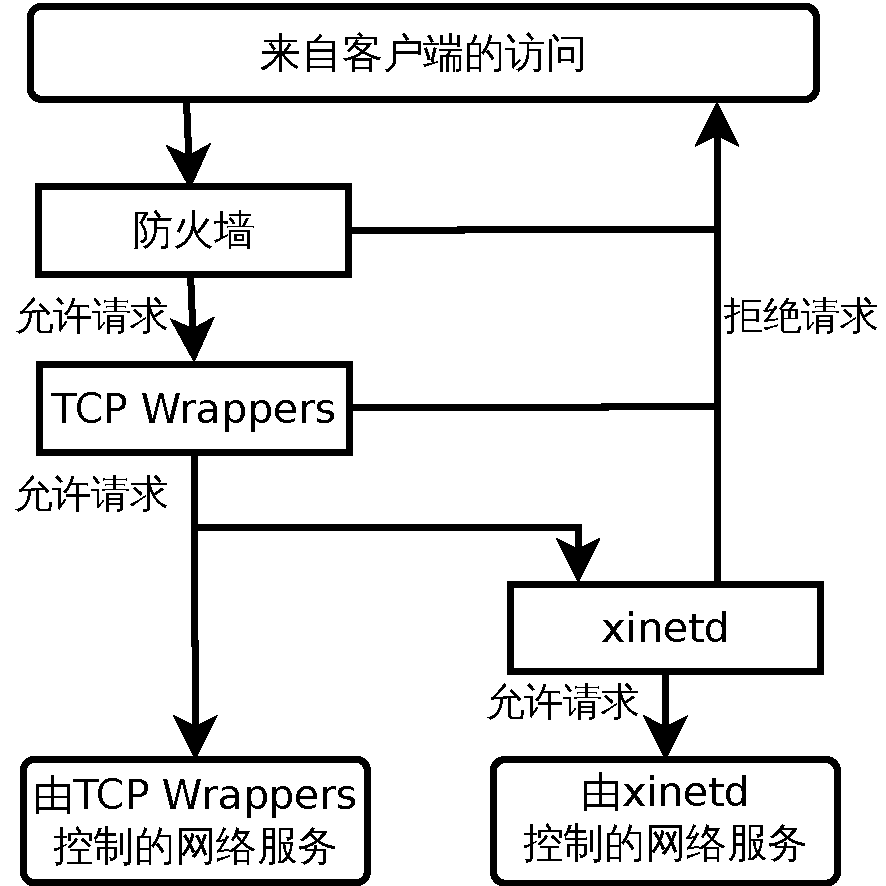
\includegraphics[width=.9\linewidth]{img/net-access.pdf}
\end{center}
\end{column}
\end{columns}
\end{frame}
\begin{frame}[fragile]
\frametitle{TCP Wrappers(1)}
\label{sec-7-3}
\begin{itemize}

\item 要开放一个本地系统以从远程系统访问时应遵循的原则:
\label{sec-7-3-1}%
\begin{enumerate}
\item 只对你允许访问的系统开放本地系统
\item 只允许每个远程系统访问你让它访问的数据
\item 只允许每个远程系统以适当的方式(只读、读写、只写)访问数据
\end{enumerate}

\item TCP Wrapper以/etc/hosts.allow和/etc/hosts.deny文件控制对系统网络服务的访问,可用于链接到libwrap库的任何守护进程。\\
\label{sec-7-3-2}%
\begin{minted}[]{bash}
ldd /usr/sbin/sshd | grep libwrap #查看sshd是否链接libwrap库
\end{minted}

\item 由TCP Wrappers控制的服务并不缓存主机访问文件中的规则,因此对hosts.allow和hosts.deny的配置修改立即生效,无需重启系统或网络服务。
\label{sec-7-3-3}%
\end{itemize} % ends low level
\end{frame}
\begin{frame}
\frametitle{TCP Wrappers(2)}
\label{sec-7-4}
\begin{columns}
\begin{column}{0.5\textwidth}
\begin{itemize}

\item hosts.allow和hosts.deny文件格式
\label{sec-7-4-1}%
\begin{itemize}

\item 服务列表:客户列表[:命令]
\label{sec-7-4-1-1}%
\end{itemize} % ends low level

\item 客户端请求访问某个服务时,按照下列顺序进行访问控制:
\label{sec-7-4-2}%
\begin{enumerate}
\item 如果服务进程/客户端对匹配hosts.allow中的一行,允许访问
\item 否则,如果服务进程/客户端对匹配hosts.deny中一行,拒绝访问
\item 否则,如果在hosts.allow和hosts.deny中均无匹配,允许访问
\end{enumerate}
\end{itemize} % ends low level
\end{column}
\begin{column}{0.5\textwidth}
%% 流程图
\label{sec-7-4-3}

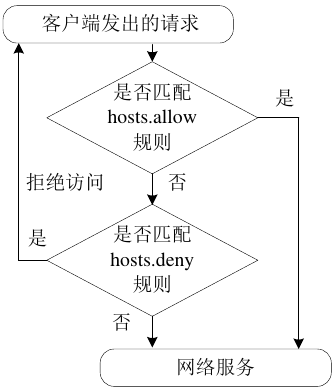
\includegraphics[width=.9\linewidth]{img/tcpwrapper.png}
\end{column}
\end{columns}
\end{frame}
\begin{frame}[fragile]
\frametitle{TCP Wrappers(3)}
\label{sec-7-5}
\begin{itemize}

\item 示例:
\label{sec-7-5-1}%
\begin{exampleblock}{/etc/hosts.deny}
\label{sec-7-5-1-1}


\begin{minted}[]{bash}
ALL:ALL:echo '%c try to connect %d - blocked' \
>>/var/log/tcpwrappers.log  #默认拒绝所有访问
\end{minted}
\end{exampleblock}
\begin{block}{/etc/hosts.allow}
\label{sec-7-5-1-2}


\begin{minted}[]{bash}
sshd:ALL         #允许从任何系统连接sshd
in.telnet:LOCAL  #允许从本域连接telnet
in.telnet:192.168.56.* 127.0.0.1 #允许指定ip连接telnet
#允许172.16网段中除172.16.251.105之外所有主机访问telnet
in.telnetd: 172.16. EXCEPT 172.16.251.105
#仅允许192.168.56.1访问telnet服务
in.telnetd:ALL EXCEPT 192.168.56.1:deny
\end{minted}
\end{block}
\end{itemize} % ends low level
\end{frame}
\begin{frame}
\frametitle{xinetd超级服务(1)}
\label{sec-7-6}
\begin{itemize}

\item xinetd本身是一个独立运行的服务,它能够同时监听多个指定的端口,在接受用户请求时,能够根据用户请求的端口不同,启动不同的网络服务进程来处理这些用户请求。
\label{sec-7-6-1}%
\begin{itemize}

\item 可以将xinetd看作是一个管理启动服务的服务器,它决定将一个客户请求交给哪个程序处理,然后启动相应的进程,完成服务请求后,再结束该进程的运行,以减少对系统资源的占用。
\label{sec-7-6-1-1}%
\end{itemize} % ends low level

\item 理论上任何服务都可以使用xinetd。但是,对于访问量大、经常出现并发访问的服务,xinetd要频繁启动对应的进程,反而会影响系统性能。因此,xinetd主要用于管理系统中不频繁使用的服务。
\label{sec-7-6-2}%
\end{itemize} % ends low level
\end{frame}
\begin{frame}
\frametitle{xinetd超级服务(2)}
\label{sec-7-7}
%% 示意图
\label{sec-7-7-1}

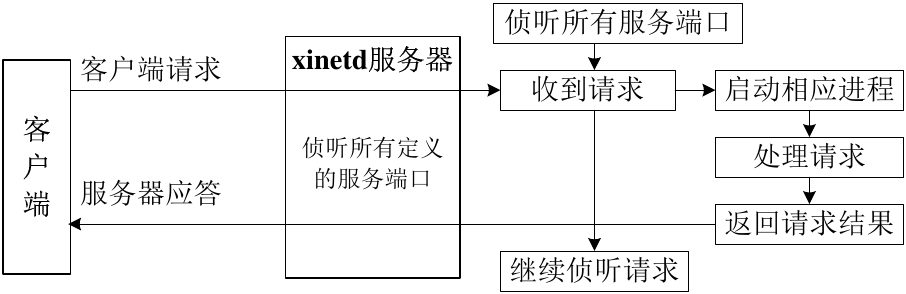
\includegraphics[width=.9\linewidth]{img/xinetd.png}
\end{frame}
\begin{frame}
\frametitle{xinetd超级服务(3)}
\label{sec-7-8}
\begin{itemize}

\item 由于xinetd本身是由TCP Wrappers控制的服务,因而对其管理的服务进行访问控制时,会同时用TCP Wrappers和xinetd控制机制。
\label{sec-7-8-1}%

\item 连接由xinetd控制的一个网络服务时,会按照以下步骤实现访问控制:
\label{sec-7-8-2}%
\begin{enumerate}
\item xinetd守护进程通过调用libwrap.a库来检查TCP Wrappers主机访问规则。
\item xinetd守护进程检查其本身的访问控制规则,包括xinetd服务和被请求的服务的控制规则。
\item 连接建立后,xinetd就不再参与客户端和服务器之间的通信。
\end{enumerate}
\end{itemize} % ends low level
\end{frame}
\begin{frame}
\frametitle{xinetd超级服务(4)}
\label{sec-7-9}
\begin{itemize}

\item 全局配置文件/etc/xinetd.conf
\label{sec-7-9-1}%
\begin{itemize}

\item 全局配置文件/etc/xinetd.conf包含一般的设置,这些设置影响xinetd所控制的每一项服务。
\label{sec-7-9-1-1}%

\item xinetd服务第一次启动时读取该文件设置信息,所以要想使修改的配置起作用,还需要重新启动xinetd服务。
\label{sec-7-9-1-2}%
\end{itemize} % ends low level

\item 特定服务配置目录/etc/xinetd.d/
\label{sec-7-9-2}%
\begin{itemize}

\item xinetd将所控制的每项服务的配置都储存在一个独立的文件中,这样更便于管理员分别定制。
\label{sec-7-9-2-1}%

\item 每项服务的配置文件位于/etc/xinetd.d/目录中,以服务的名称命名,文件格式与/etc/xinetd.conf相同。
\label{sec-7-9-2-2}%

\end{itemize} % ends low level
\end{itemize} % ends low level
\end{frame}

\end{document}
